%%%%%%%% ICML 2023 EXAMPLE LATEX SUBMISSION FILE %%%%%%%%%%%%%%%%%

\documentclass{article}

% Recommended, but optional, packages for figures and better typesetting:
\usepackage{microtype}
%\usepackage{graphicx}
\usepackage{graphics, graphicx}
\usepackage{float}
\usepackage{subfig}
%\usepackage{subfigure}
\usepackage{booktabs} % for professional tables

\usepackage{tikz}
% Corporate Design of the University of Tübingen
% Primary Colors
\definecolor{TUred}{RGB}{165,30,55}
\definecolor{TUgold}{RGB}{180,160,105}
\definecolor{TUdark}{RGB}{50,65,75}
\definecolor{TUgray}{RGB}{175,179,183}

% Secondary Colors
\definecolor{TUdarkblue}{RGB}{65,90,140}
\definecolor{TUblue}{RGB}{0,105,170}
\definecolor{TUlightblue}{RGB}{80,170,200}
\definecolor{TUlightgreen}{RGB}{130,185,160}
\definecolor{TUgreen}{RGB}{125,165,75}
\definecolor{TUdarkgreen}{RGB}{50,110,30}
\definecolor{TUocre}{RGB}{200,80,60}
\definecolor{TUviolet}{RGB}{175,110,150}
\definecolor{TUmauve}{RGB}{180,160,150}
\definecolor{TUbeige}{RGB}{215,180,105}
\definecolor{TUorange}{RGB}{210,150,0}
\definecolor{TUbrown}{RGB}{145,105,70}

% hyperref makes hyperlinks in the resulting PDF.
% If your build breaks (sometimes temporarily if a hyperlink spans a page)
% please comment out the following usepackage line and replace
% \usepackage{icml2023} with \usepackage[nohyperref]{icml2023} above.
\usepackage{hyperref}
\usepackage{wrapfig}

% Attempt to make hyperref and algorithmic work together better:
\newcommand{\theHalgorithm}{\arabic{algorithm}}

\usepackage[accepted]{icml2023}

% For theorems and such
\usepackage{amsmath}
\usepackage{amssymb}
\usepackage{mathtools}
\usepackage{amsthm}

% if you use cleveref..
\usepackage[capitalize,noabbrev]{cleveref}

%%%%%%%%%%%%%%%%%%%%%%%%%%%%%%%%
% THEOREMS
%%%%%%%%%%%%%%%%%%%%%%%%%%%%%%%%
\theoremstyle{plain}
\newtheorem{theorem}{Theorem}[section]
\newtheorem{proposition}[theorem]{Proposition}
\newtheorem{lemma}[theorem]{Lemma}
\newtheorem{corollary}[theorem]{Corollary}
\theoremstyle{definition}
\newtheorem{definition}[theorem]{Definition}
\newtheorem{assumption}[theorem]{Assumption}
\theoremstyle{remark}
\newtheorem{remark}[theorem]{Remark}

% Todonotes is useful during development; simply uncomment the next line
%    and comment out the line below the next line to turn off comments
%\usepackage[disable,textsize=tiny]{todonotes}
\usepackage[textsize=tiny]{todonotes}


% The \icmltitle you define below is probably too long as a header.
% Therefore, a short form for the running title is supplied here:
\icmltitlerunning{Into the minds of gamers -\\
Extracting player preferences from steam reviews}

%\setlength{\abovecaptionskip}{15pt plus 3pt minus 2pt}

\begin{document}

\twocolumn[
\icmltitle{Into the minds of gamers -\\
Extracting player preferences from steam reviews}

% It is OKAY to include author information, even for blind
% submissions: the style file will automatically remove it for you
% unless you've provided the [accepted] option to the icml2023
% package.

% List of affiliations: The first argument should be a (short)
% identifier you will use later to specify author affiliations
% Academic affiliations should list Department, University, City, Region, Country
% Industry affiliations should list Company, City, Region, Country

% You can specify symbols, otherwise they are numbered in order.
% Ideally, you should not use this facility. Affiliations will be numbered
% in order of appearance and this is the preferred way.
\icmlsetsymbol{equal}{*}

\begin{icmlauthorlist}
\icmlauthor{Michael Pasch}{equal,first}
\icmlauthor{Nikolas Schäfer}{equal,second}
\icmlauthor{Isabel Schüle}{equal,third}
\end{icmlauthorlist}

% fill in your matrikelnummer, email address, degree, for each group member
\icmlaffiliation{first}{Matrikelnummer 6084103, michael.pasch@student.uni-tuebingen.de, BSc Computer Science}
\icmlaffiliation{second}{Matrikelnummer 4208976, nikolas.schaefer@student.uni-tuebingen.de, MSc Computer Science}
\icmlaffiliation{third}{Matrikelnummer 6222071, isabel.schuele@student.uni-tuebingen.de, MSc Computer Science}

% You may provide any keywords that you
% find helpful for describing your paper; these are used to populate
% the "keywords" metadata in the PDF but will not be shown in the document
\icmlkeywords{Machine Learning, ICML}

\vskip 0.3in
]

% this must go after the closing bracket ] following \twocolumn[ ...

% This command actually creates the footnote in the first column
% listing the affiliations and the copyright notice.
% The command takes one argument, which is text to display at the start of the footnote.
% The \icmlEqualContribution command is standard text for equal contribution.
% Remove it (just {}) if you do not need this facility.

%\printAffiliationsAndNotice{}  % leave blank if no need to mention equal contribution
\printAffiliationsAndNotice{\icmlEqualContribution} % otherwise use the standard text.

\begin{abstract}
%Put your abstract here. Abstracts typically start with a sentence motivating why the subject is interesting. Then mention the data, methodology or methods you are working with, and describe results. 
User reviews hold valuable information not only for consumers but also for the business offering the product. We research the usefulness of information that can be extracted via automated processing of computer game reviews. Using a pretrained NLP-model we visualize the correlation between reviews of similar rating and evaluate the frequency of meaningful words in a wordcount-graph yielding information about which words and word-combinations carry a positive or negative connotation. We show that the information extracted in this automated fashion provides valuable insights into the preferences and priorities of players as well as general pitfalls to avoid when publishing games. 
\end{abstract}


\section{Introduction}\label{sec:intro}

%Motivate the problem, situation or topic you decided to work on. Describe why it matters (is it of societal, economic, scientific value?). Outline the rest of the paper (use references, e.g.~to \Cref{sec:methods}: What kind of data you are working with, how you analyse it, and what kind of conclusion you reached. The point of the introduction is to make the reader want to read the rest of the paper.
The video game industry is an ever growing business sector which generated $249.58$ billion US\$ in revenue in 2023 alone \cite{game_revenue}. To be able to profit off this sector, video game developers and publishers have to make each game a success as a badly received game results not only in a short-term loss in revenue, but player disappointment might also cause the customer base to shrink for future projects. A studio closing over one unsuccessful game is not that uncommon \cite{forspoken_game_studio}.
\\This makes customer feedback via reviews a valuable source of information for developers and publishers to learn about potential pitfalls and positively regarded features in video games. Past research has shown that game reviews often focus not only on personal player experience, but also contain explicit comments about game contents, bugs or suggestions for the publishers \cite{linbezemerzouhassan}. Therefore, player feedback provides valuable information on a rich set of topics, making it relevant not only for potential buyers, but also for developers \cite{zagalladdjohnson}. However, manually reading and evaluating thousands or tens of thousands of reviews is generally not feasible.\\
We analyze textual game reviews acquired from the popular distribution platform Steam \cite{steam_website} with a pretrained NLP model, to find correlation between positive and negative feedback (\ref{fig:corr-plot}). Additionally, we analyze the occurrences of common keywords and word combinations in these reviews to attain a better understanding of the players' preferences (\ref{fig:wordcount_pos}, \ref{fig:wordcount_neg}). Our code can be found at \cite{gitrepo}.
%The outline of this work is as follows: In ch2 we first explain our methodology in how we approached the mentioned tasks, followed by a presentation of our results in ch3 which we then discuss in ch4 before we close with some final remarks in ch5 (restructure this part!).

\begin{figure}%[H]
    \centering
    \includegraphics[width=9cm]{../fig/The_Elder_Scrolls_V_matrix.pdf}
    \vspace{-4\baselineskip}
    \caption{Visualization of correlation between the mean wordvectors extracted by the NLP for each review from the game The Elder Scrolls V. Each row/column represents one review with the negative reviews (0-3649) separated from the positive ones by a white line. The plot shows stronger correlation between reviews of same rating (especially neg/neg). }
    %\vspace{\baselineskip}
    %\setlength\belowcaptionskip{-10pt}
    %\setlength\intextsep{0pt}
    \label{fig:corr-plot}
\end{figure}


\newpage
\section{Data and Methods}\label{sec:methods}

%In this section, describe \emph{what you did}. Roughly speaking, explain what data you worked with, how or from where it was collected, it's structure and size. Explain your analysis, and any specific choices you made in it. Depending on the nature of your project, you may focus more or less on certain aspects. If you collected data yourself, explain the collection process in detail. If you downloaded data from the net, show an exploratory analysis that builds intuition for the data, and shows that you know the data well. If you are doing a custom analysis, explain how it works and why it is the right choice. If you are using a standard tool, it may still help to briefly outline it. Cite relevant works. You can use the \verb|\citep| and \verb|\citet| commands for this purpose \citep{mackay2003information}.

For our research we use a dataset of gamereviews \cite{first_dataset} collected in 2015 from the Steam website which includes feedback for eleven popular games with a sample-size between 1.500 and 13.000 reviews per game. The data is already filtered to only include reviews written in English. Of the features available in the dataset we use the review text as well as the game rating, which is a binary integer value of either 0 (negative) or 1 (positive).
%A first look at the data revealed that the dataset has a strong bias as most of the games have an overwhelming positive score.
\\As the scope of this paper is limited we focus on a subset of these games to do a more in depth analysis. The games belong to different genres, therefore we refrain from averaging over reviews of different games with different player bases. Instead, from a game developer's point of view, it is much more insightful to dive into the feedback of the player base of one particular game and try to grasp the opinion of those players over the large number of reviews.\\
We chose the games included in our analysis with the goal of covering a broad spectrum of popularity from negative to positive as listed in table \ref{tab:gamenumbers}.\\ 
The positive end of the spectrum is covered by 'Counter Strike Global Offensive' and 'Garry’s Mod' while 'Grand Theft Auto V' and 'The Elder Scrolls V' place towards the middle of the scale with a mixed total score. To include a sample with mostly negative feedback we supplemented our reviews with data from 'Fallout 4' taken from a second dataset \cite{second_dataset}. This was necessary because our original dataset has a strong positive bias as all games have a positive ratio of 47.4\% or more. \\
Before we analyze the textual data we apply some pre-processing by first converting all text to lowercase to prevent the same word being treated differently because of case-sensitivity. In a second step we remove a large amount of 'stopwords' from the review-texts, which are words that are considered to carry no or little relevant information in regard to the core topic of a sentence (for example pronouns or prepositions). To this end we utilize the python module many\_stop\_words \cite{many_stop_words}, which provides 894 stopwords for the English language. Next, we use the wordnet-model of the NLTK library \cite{bird2009natural} to lemmatize all verbs, adjectives and nouns. Lemmatization describes the process of reducing words to their dictionary form (called lemma), so that their different inflections are not treated separately. On top of that we remove all special characters from the text to sort out reviews consisting of ASCII-Art. Finally, we drop all entries in our dataframe which end up empty after application of the aforementioned filters.\\
After some basic inspection of the data we investigated our first hypothesis according to which the content of reviews should be correlated with those of the same rating. To test this we made use of the python library 'spaCy' \cite{spacy} which provides pre-trained models for natural language processing. With the English language model 'en\_core\_web\_lg' we used a feature of this library allowing us to transform the text of an entire review into a single vector. This works by turning every single word into the internal representation the model has learned for it, and taking the mean of those wordvectors. Since vectors of words of similar meaning should be close to each other for a given metric, we assumed that this also holds true for the mean vectors of reviews, if those discuss similar content. By computing the  correlation coefficient matrix for those vectors however, we found that this only holds true for some of the games, such as 'The Elder Scrolls V', as shown in figure \ref{fig:corr-plot}. For other games we could not observe a clear correlation.\\ 
The cause of this inconsistent correlation might on the one hand be the method itself, as the mean-vectors of documents of different sizes extracted by a model trained on general text data (not game reviews specifically) might not be meaningful. On the other hand the reviews sharing the same sentiment towards a game might do so for totally different reasons.\\
To take a closer look at the reasons for a certain rating, we then separately analyzed the positive and negative textual data for frequency of single words (uni-gram), as well as combinations of two words (bi-gram) using the python library 'sklearn' \cite{Scikit}. We filter the uni-grams and bi-grams for their appearance frequency relative to the number of reviews, with a threshold of $8 \ \%$. That way, we can find the keywords with the highest relevance across all reviews from a specific game.\\%TODO: Lemmatization
%In this report we focus only on this subset of games because we specifically do not want to average over reviews on many different games with different player bases. Instead, from a game developer's point of view, it is much more fruitful to dive into the feedback of the player base of one particular game and try to grasp the opinion of those players over the large number of reviews.

%vectorizer, tokinization, player-community(quirks), resources 

\begin{table}[htb]
\resizebox{\columnwidth}{!}{%
\begin{tabular}{l|c|c}
    \textbf{Game} & \textbf{Reviews} & \textbf{Positive ratio}  \\
    \hline\hline
    Grand Theft Auto V & 11190 & $66.5 \ \%$\\
    The Elder Scrolls V & 7165 & $47.4 \ \%$\\
    Counter Strike Global Offensive & 5837 & $95.0 \ \%$\\
    Garry's Mod & 6204 & $99.1 \ \%$\\
    Fallout 4 & 6120 & $34.1 \ \%$
\end{tabular}
}
\caption{The five games we analyzed in detail. The middle column shows the number of reviews from the respective game. In order to look at games from a range of popularity, we compared the number of positive reviews (rated with $1$) to the total number of reviews. The third column shows this ratio.}
\vspace{+2\baselineskip}
\label{tab:gamenumbers}
\end{table}

\begin{figure*}[!h]
  \centering
  \subfloat[\label{fig:wordcount_pos}]{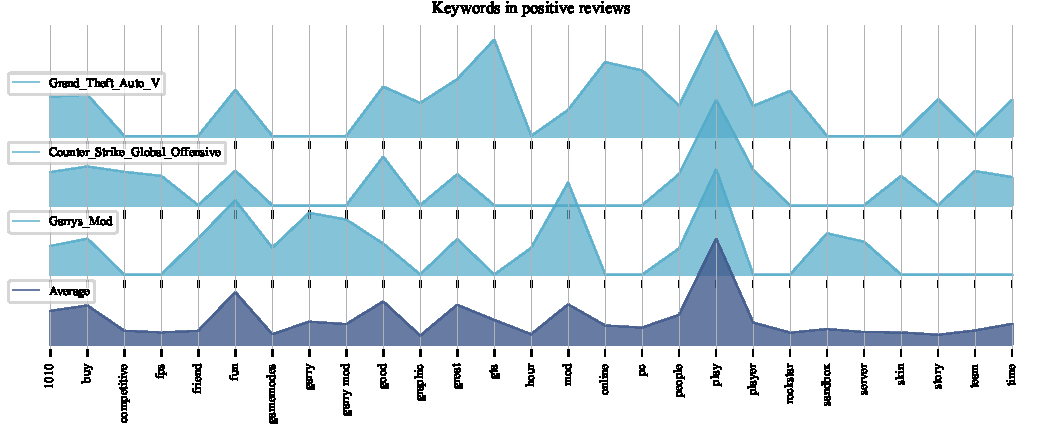
\includegraphics{../fig/wordcount_plot_report_pos.pdf}}
  
    \par
  %\vspace{5mm}

\subfloat[\label{fig:wordcount_neg}]{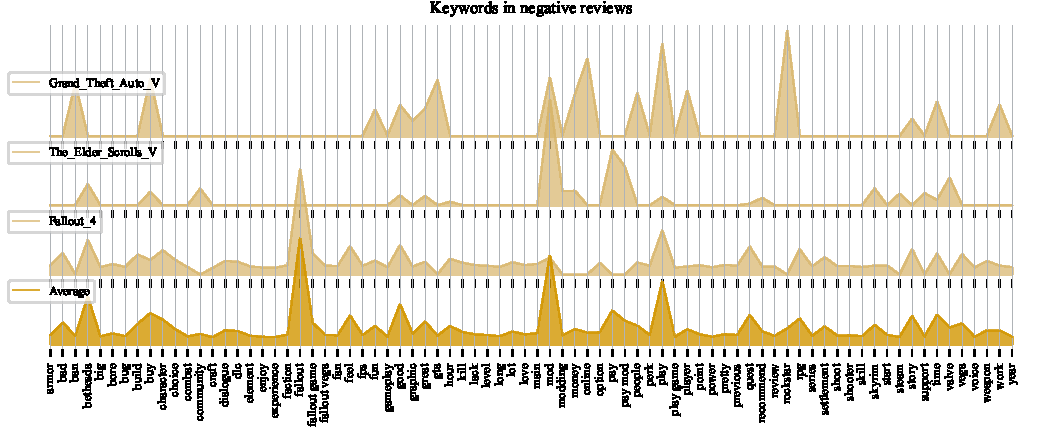
\includegraphics{../fig/wordcount_plot_report_neg.pdf}}
  \caption{\textbf{Top}: Keywords with highest relative appearance in selected games with a high number of positive reviews. \textbf{Bottom}: Keywords with highest relative appearance in selected games with a high number of negative reviews. The y-axes are scaled individually to make the appearance of the keywords better visible. The bottom row of each plot shows the average over the three games above.}
    \label{fig:wordcount}
\end{figure*}
%Grand_Theft_Auto_V: choosing 11190 out of 11190 reviews. Positive ratio: 0.66514745308311
%Counter_Strike_Global_Offensive: choosing 5837 out of 5837 reviews. Positive ratio: 0.9498029809833819
%Garrys_Mod: choosing 6204 out of 6204 reviews. Positive ratio: 0.9912959381044487
%Grand_Theft_Auto_V: choosing 11190 out of 11190 reviews. Positive ratio: 0.66514745308311
%The_Elder_Scrolls_V: choosing 6258 out of 6258 reviews. Positive ratio: 0.4741131351869607
%Fallout_4: choosing 6120 out of 6120 reviews. Positive ratio: 0.3411764705882353
%Table \ref{tab:gamenumbers} shows the five games we analyzed in detail. The middle column shows the number of reviews from the respective game. In order to look at games from a range of popularity, we compared the number of positive reviews (rated with $1$) to the total number of reviews. The third column shows this ratio.

%With Grand Theft Auto V and The Elder Scrolls V we selected two games with around half of the reviews being positive. Counter Strike Global Offensive and Garry's Mod both received an overwhelming amount of positive feedback. Fallout 4 on the other hand is the only game with a much higher number of negative reviews, stemming from the additional dataset [cite] as our main dataset did not include any game with a similar ratio.\\

To avoid false balancing, our results in the following section (\ref{sec:results}) show only the analysis of positive reviews from Counter Strike Global Offensive and Garry's Mod, whereas we focus on negative reviews from The Elder Scrolls V and Fallout 4. For Grand Theft Auto V, we visualize positive and negative feedback.
%In the course of our analysis, we split each review from each game into single words and filtered those for stopwords [explain!] and special characters. This allowed us to filter out ASCII art (which consists only of special characters) and words that do not carry meaning on their own. We then analyze the resulting sequences of words for frequency of single words, as well as combinations of two words. Finally, we filter the single words and 2-word-combinations for their appearance frequency relative to the number of reviews from that specific game, with a threshold of $8 \ \%$. That way, we can find the keywords with the highest relevance across all reviews from a specific game.\\


% This is the template for a figure from the original ICML submission pack. In lecture 10 we will discuss plotting in detail.
% Refer to this lecture on how to include figures in this text.
% 
% \begin{figure}[ht]
% \vskip 0.2in
% \begin{center}
% \centerline{\includegraphics[width=\columnwidth]{icml_numpapers}}
% \caption{Historical locations and number of accepted papers for International
% Machine Learning Conferences (ICML 1993 -- ICML 2008) and International
% Workshops on Machine Learning (ML 1988 -- ML 1992). At the time this figure was
% produced, the number of accepted papers for ICML 2008 was unknown and instead
% estimated.}
% \label{icml-historical}
% \end{center}
% \vskip -0.2in
% \end{figure}
\newpage
\section{Results}\label{sec:results}


%In this section outline your results. At this point, you are just stating the outcome of your analysis. You can highlight important aspects (``we observe a significantly higher value of $x$ over $y$''), but leave interpretation and opinion to the next section. This section absoultely \emph{has} to include at least two figures.

We visualize our main findings in figures \ref{fig:wordcount_pos} and \ref{fig:wordcount_neg} by plotting the relative frequency of the filtered keywords for the selected games.\\
Figure \ref{fig:wordcount_pos} shows the most frequently used words and word combinations in the positive reviews of the games Grand Theft Auto V, Counter Strike Global Offensive and Garry's Mod. Figure \ref{fig:wordcount_neg} visualizes the most frequently used words and word combinations in the negative reviews of Grand Theft Auto V, The Elder Scrolls V and Fallout 4. Additionally, each plot contains the average frequency over the respective games.\\
One prominent finding is that the number of keywords in the plots for positive reviews is much smaller than for negative reviews, even though the keywords were filtered with the same threshold of relative appearance. This suggests that the players leaving negative reviews focus more on specific aspects and shortcomings of a game than the players leaving positive reviews.\\
The keywords for the positive reviews in figure \ref{fig:wordcount_pos} further support this theory. There are several keywords with a high appearance in all of the games, namely "1010", which comes from the expression "10/10" with the special character removed; "buy", "fun", "good", "great" and "play". All of those keywords are positively associated, but very general and not very informative.\\
The analysis becomes more interesting when we focus on peaks for the specific games, such as "graphic", "online", "pc", "people" and "story" for Grand Theft Auto V. Those keywords imply that this particular game was rated positively because of its visuals, the story and the online gameplay with other people. On top of that the publisher "rockstar" appears in a large number of positive reviews.\\
For Counter Strike Global Offensive, the reviewers seem to be especially satisfied with the "competitive" gameplay in teams, and the different "skins" for the in game items. The third game, Garry's Mod, which is also a multiplayer game, received a lot of positive reviews mentioning the different "gamemodes", the other "people" (highlighting the social aspect of the game),  and the fact that it is a "sandbox" game which gives the players a lot of options to shape the gameplay according to their ideas.\\
Looking at the keywords in negative reviews in figure \ref{fig:wordcount_neg} the peaks for the individual games are generally more sparse than for the positive reviews.
%The most prominent reasons why a game has a lot of negative reviews are the keywords "graphics", "money", "online", "people" and "rockstar" for Grand Theft Auto V. showing that some of the points in positive reviews reappear in negative reviews of the same game.In this case the publisher, "rockstar", appears much more frequently in relation to the other keywords, when comparing to the positive reviews of the same game.\\
For Grand Theft Auto V the keywords "online" and "people" indicate that the social aspect of the game was not well received by all players. The keyword "ban" implies either a dissatisfaction with players being deliberately banned, or not being banned fast enough for misbehavior. The keyword "rockstar" not only appears in the positive but also in the negative reviews, implying that the players have split opinions on this publisher.\\
A relevant keyword in fig \ref{fig:wordcount_neg} is "bethesda", which appears frequently in reviews for The Elder Scrolls V and Fallout 4. Bethesda is the publisher of those games, the prevalent mentioning in the review texts suggests that the video game community is very aware of the company behind a respective game and negative sentiment towards the product also reflects back on its publisher.\\
Reviewers of The Elder Scrolls V mentioned the player "community" and the "support" frequently in negative reviews. Especially interesting however are the keywords connected to "mod". "Mod" stands for modification, and describes modifications made to games by the player community. Mods are usually published by the community to be used for free by the other players. The Elder Scrolls V is famous for its big modding community which gives players options to change the look and feel of the game completely. In 2015 however, Bethesda and Steam introduced purchasable mods for a short time \cite{paid_mods} which led to a big backlash from the community. This event is clearly visible in the plot with the frequent appearance of keywords like "bethesda", "mod", "pay" and "pay mod". Again we can see that the gaming community tends to connect their dissatisfaction directly with the publisher which they see responsible.\\
For the third game, Fallout 4, the review keywords suggest that a lot of reviewers were unsatisfied with the "characters", "feel", "quests" and "story" of the game.
%To summarize our results, the plots show that there is more detailed information to find in negative reviews compared to positive reviews. Looking into the frequent keywords for specific games however, it is still possible for a game developer to find aspects of a published game that the community really enjoys, like sandbox games, the story or the game's visuals. When it comes to negative reviews our analysis shows that the player base is very aware of the publisher of the respective game, and tends to connect not only bad aspects in the actual gameplay (like the characters or the story) but especially badly received decisions involving the game, like the paid mods in The Elder Scrolls V, directly to the publisher. This shows the importance of any game developer knowing their community well and learn from past mistakes. Analyses of released games with the tools we introduced here, can give a solid impression of what pitfalls to avoid.
%Skyrim: bethesda, community, mod, modding, mods, paid, paid mods, skyrim, steam, valve
%Fallout: bethesda, character, fallout vegas (spin-off released earlier), quests, story



\section{Discussion \& Conclusion}\label{sec:conclusion}

%Use this section to briefly summarize the entire text. Highlight limitations and problems, but also make clear statements where they are possible and supported by the analysis. 
Our analysis shows that a game's reviews provide a lot of interesting information about the game. We found that negative reviews tend to contain more explicit information, as the keywords we extracted from positive reviews are mostly kept general, and draw less connections to specific aspects of the game. Nevertheless we found interesting keywords such as "sandbox", "competitive" or "online" that show the players' appreciation of certain features.\\
The negative reviews show that the dissatisfaction with controversial decisions of the publisher has a direct influence on the sentiment of the reviews, for example the paid mods introduced for The Elder Scrolls V. The frequent mentioning of the publisher shows that the sentiment towards a game is interlinked with the reputation of the publisher. Additionally, the keywords we extracted from negative reviews highlight shortcomings of particular games like the story, characters or gameplay-mechanics.\\
Despite our initial analysis of the correlation between reviews with the same rating producing inconsistent results, the keyword-analysis shows that it is possible to extract valuable information from a large number of game reviews. This qualitative analysis gives a good overview over topics that are important to the player base of a video game, and allows game developers to find out what aspects of a released game were received well or criticized.\\
Because we only focus on the frequency of keywords and not on their semantic context within the sentence, as would be possible with a large language model, we have to restrain our conclusions to assumptions on the real intent of the reviewers. 
Nevertheless we are convinced that developers and publishers can profit a lot from this kind of evaluation of game reviews and draw useful insights on what aspects can make a game a success or failure.
%This problem occurs, when there is no really unique aspect to a game and therefore the most used words for both sides are relatively similar. With a finer evaluation there might be a more pronounced difference, but in that case the number of keywords gets way too high to do a reasonable analysis or visualization.\\
%Moreover there is often a problem with the ratio between positive and negative reviews, in most cases there are far more positive than negative reviews, which makes comparison difficult. To remedy this we even had to add games from another dataset.\\
%The correlation matrices of the different games, which we did to see if there was some kind of correlation between the text of positive and negative reviews are also quite unexpected. We expected to see quite a strong correlation between all the positive reviews and all the negative reviews. But most of the time this difference is not really visible, if there at all. This is why we focused primarily on the numbers of different keywords, rather than the correlations.\\


\section*{Contribution Statement}
%initial analysis of data                        (all)
%textdata preprocessing and analysis (code)       Nikolas
%finding resources (related work)/ literature review (all)
%correlation analysis (plot)                     (Michael)
%wordcount/frequency plot                        (Isabell)
%report text                                     (all)
%github repo + readme                            (Isabell)

Nikolas Schäfer implemented the code for the pre-processing and analysis of the review texts.
Michael Pasch constructed the correlation plot.
Isabel Schüle created and maintained the github repo and produced the visualizations for the keyword plots.
All authors jointly performed the initial analysis of the data, reviewed relevant resources and literature, and wrote the report text.

%Explain here, in one sentence per person, what each group member contributed. For example, you could write: Max Mustermann collected and prepared data. Gabi Musterfrau and John Doe performed the data analysis. Jane Doe produced visualizations. All authors will jointly wrote the text of the report. Note that you, as a group, a collectively responsible for the report. Your contributions should be roughly equal in amount and difficulty.

%\section*{Notes} 

%Your entire report has a \textbf{hard page limit of 4 pages} excluding references. (I.e. any pages beyond page 4 must only contain references). Appendices are \emph{not} possible. But you can put additional material, like interactive visualizations or videos, on a githunb repo (use \href{https://github.com/pnkraemer/tueplots}{links} in your pdf to refer to them). Each report has to contain \textbf{at least three plots or visualizations}, and \textbf{cite at least two references}. More details about how to prepare the report, inclucing how to produce plots, cite correctly, and how to ideally structure your github repo, will be discussed in the lecture, where a rubric for the evaluation will also be provided.
%\onecolumn 
\newpage
\bibliography{bibliography}
\bibliographystyle{icml2023}

\end{document}


% This document was modified from the file originally made available by
% Pat Langley and Andrea Danyluk for ICML-2K. This version was created
% by Iain Murray in 2018, and modified by Alexandre Bouchard in
% 2019 and 2021 and by Csaba Szepesvari, Gang Niu and Sivan Sabato in 2022.
% Modified again in 2023 by Sivan Sabato and Jonathan Scarlett.
% Previous contributors include Dan Roy, Lise Getoor and Tobias
% Scheffer, which was slightly modified from the 2010 version by
% Thorsten Joachims & Johannes Fuernkranz, slightly modified from the
% 2009 version by Kiri Wagstaff and Sam Roweis's 2008 version, which is
% slightly modified from Prasad Tadepalli's 2007 version which is a
% lightly changed version of the previous year's version by Andrew
% Moore, which was in turn edited from those of Kristian Kersting and
% Codrina Lauth. Alex Smola contributed to the algorithmic style files.

